\section{Persona Induction: Comparison and Controls}\label{sec:appendix-induction-sweeps}

This appendix compares LoRA-based persona induction against system-prompt, prefix-tuning adaptors and activation-space baselines, supplies the per-method coefficient sweeps that pin down the headline coefficients, and reports cross-trait and cross-control replications.

\textbf{Setup.} All experiments share the same configuration. Llama-3.1-8B-Instruct is the assistant model; gpt-4.1-mini is the user-simulator following a generic ``curious, engaged user'' template (the \texttt{typical\_user} template, reproduced in full in Section~\ref{sec:appendix-induction-assets}). At each (method, direction) point we compare four interventions: \emph{(i)} no intervention (baseline); \emph{(ii)} a system prompt instructing the desired trait, using the canonical OCEAN-definition prose described in Section~\ref{sec:appendix-induction-assets}; \emph{(iii)} a trait LoRA; and \emph{(iv)} activation capping along the trait axis. The LoRA adapters are the canonical paired-DPO versions trained per \Cref{sec:training-loras,sec:constitutions}; activation-capping axes are recomputed per direction against those same adapters. The headline E$\uparrow$ comparison (Figure~\ref{fig:eplus-induction}) runs 40 prompts $\times$ 3 rollouts $\times$ 15 turns per condition ($= 1800$ assistant messages); the rest of the appendix uses 10 prompts $\times$ 2 rollouts $\times$ 15 turns per condition ($= 300$ assistant messages). The smaller scale produces noisier per-condition estimates and is a known limitation; the trends are clear enough to support the qualitative claims we make from them. Bootstrap 95\% CIs are computed across the per-prompt $\times$ per-rollout sample. The assistant runs at temperature $0.7$ with no top-$p$ filtering (Section~\ref{sec:appendix-induction-temperature} contrasts this with the default of $1.0$). Seed prompts are drawn deterministically from a 299-prompt neutral psychometric pool (a curated extension of the assistant-axis questions of~\citet{lu2026assistant}; sample prompts in Section~\ref{sec:appendix-induction-assets}) using \texttt{seed=42}; the user-roleplay subsection (\ref{sec:appendix-induction-roleplay}) is the only experiment that uses scenario-driven prompts instead.

\subsection{Comparison to Activation-Space and Prompt-Based Induction}\label{sec:comparison-induction}

The single-LoRA results in Section~\ref{sec:results-single-loras} show that LoRA adapters can move models along psychometrically defined trait axes. We compare our method here against two natural baselines: a system prompt instructing the desired trait, and activation capping~\citep{lu2026assistant}, which clamps activations along a persona axis at a fixed value (see Appendix~\ref{sec:activation_capping} for reproduction details).

A short note on activation capping. The technique was introduced as a way to \emph{cap} a model's expression of an extracted persona axis at a target value, hence the name. In practice the operation is symmetric: when the model's natural projection along the axis is below the target value, capping pulls the projection \emph{up} to the target rather than holding it down. So when we use capping to induce a trait that the model does not natively express --- the case throughout this appendix --- the technique behaves as a tailored form of activation steering, with the projection itself, rather than an additive offset, as the controlled quantity. We benchmark against capping rather than additive activation steering because the prior work we compare to~\citep{lu2026assistant} uses capping along a persona axis, which is the closer analogue to applying a LoRA along a trait axis.

We frame this as a \emph{trait induction} problem: whether each method, applied to a model in its natural register on neutral prompts, can move the model into a target trait register. The LoRA and activation-capping coefficients are picked from a per-method sweep, choosing the strongest variant that does not visibly damage coherence (full sweeps in Appendix~\ref{sec:appendix-induction-sweeps-loraac}). On E$\uparrow$ (Figure~\ref{fig:eplus-induction}), the LoRA reaches the highest trait expression while preserving the highest coherence across all 15 turns; sysprompt starts near the LoRA's level but drifts down turn-by-turn as the model relaxes the instructed persona; activation capping plateaus lower and steadily loses coherence. The rest of this appendix expands on this picture: the trait-coherence Pareto frontier (Appendix~\ref{sec:appendix-induction-pareto}), cross-LoRA controls confirming the trait shift comes from the trait-shaping LoRA specifically (Appendix~\ref{sec:appendix-induction-crosslora}), the suppressor direction where all three methods plateau before reaching sysprompt's level (Appendix~\ref{sec:appendix-induction-eminus-floor}), the same comparison replicated on openness (Appendix~\ref{sec:appendix-induction-openness}), and a complementary experiment where the same LoRA is asked to \emph{hold} a trait against opposing user-side pressure rather than steer on neutral prompts (Appendix~\ref{sec:appendix-induction-drift-prevention}).

% Generated by: src_dev/visualisations/paper_main_eplus_induction.py
% Data: HF persona-cartography/monorepo — see paper/figures/MANIFEST.md
\begin{figure}[htbp]
\centering
\includegraphics[width=\linewidth]{figures/appendix/induction/fig_3_4_eplus_induction_comparison.pdf}
\caption{Per-turn extraversion (left) and coherence (right) trajectories for the four E$\uparrow$ induction methods on neutral psychometric prompts. Each cell is $40$ prompts $\times$ $3$ rollouts $\times$ $15$ turns ($1800$ assistant messages). Llama-3.1-8B-Instruct as assistant at temperature $0.7$; gpt-4.1-mini as the user-simulator. Error bars show bootstrap $95\%$ CIs over the per-prompt $\times$ per-rollout sample.}
\label{fig:eplus-induction}
\end{figure}

\subsection{Coefficient Sweeps to Select the Coefficients}\label{sec:appendix-induction-sweeps-loraac}

We sweep each method across a range of intervention strengths and pick the strongest variant that retains near-base coherence and avoids qualitative degradation visible at higher coefficients (Figure~\ref{fig:induction-method-sweeps}). On the LoRA side, trait expression climbs monotonically with coefficient and coherence stays near base throughout the sweep; we nonetheless pick coefficient $0.75$ rather than $1.00$ after reading transcripts --- at $1.00$ the model writes in an exaggerated tone (lots of capital letters, repeated exclamation marks, the same kinds of enthusiastic phrases over and over) that the coherence judge does not flag but reads as forced. On the activation capping side, trait expression also climbs monotonically but coherence drops once the fraction passes $\sim 0.5$; coefficient $0.85$ is the elbow where trait gain slows but coherence has not yet collapsed.

\begin{figure}[htbp]
\centering
\begin{subfigure}[t]{0.49\linewidth}
  \centering
  % Generated by: src_dev/visualisations/paper_appendix_induction_method_sweeps.py
  % Data: HF persona-cartography/monorepo — see paper/figures/MANIFEST.md
  \includegraphics[width=\linewidth]{figures/appendix/induction/fig_G_induction_lora_sweep.pdf}
  \caption{LoRA scale sweep.}
  \label{fig:induction-lora-sweep}
\end{subfigure}
\hfill
\begin{subfigure}[t]{0.49\linewidth}
  \centering
  % Generated by: src_dev/visualisations/paper_appendix_induction_method_sweeps.py
  % Data: HF persona-cartography/monorepo — see paper/figures/MANIFEST.md
  \includegraphics[width=\linewidth]{figures/appendix/induction/fig_G_induction_actcap_sweep.pdf}
  \caption{Activation capping fraction sweep.}
  \label{fig:induction-actcap-sweep}
\end{subfigure}
\caption{Per-method intervention-strength sweeps for E$\uparrow$ induction. Each panel shows per-turn extraversion (left) and coherence (right) for one method across its full coefficient range.}
\label{fig:induction-method-sweeps}
\end{figure}

\subsection{Trait-Coherence Pareto frontier}\label{sec:appendix-induction-pareto}

Plotting each (method, strength) point in (extraversion, coherence) space (Figure~\ref{fig:induction-pareto}) makes the trade-off direct. LoRA traces a tight curve along the top of the plot --- coherence stays near base across the entire sweep, and at coefficient $1.00$ the trait reaches $+3.64$ at coherence $8.02$. Activation capping traces a steeper trade-off: trait gain past coefficient $0.75$ comes with a clear coherence cost, and by coefficient $1.00$ coherence has dropped to $6.24$. Sysprompt sits as a single point near LoRA $0.75$ at $(+3.06, 8.43)$, with no scale knob.

Two things stand out. First, LoRA strictly dominates activation capping at every trait level above $\sim+1.5$: the two methods can reach the same trait values, but LoRA does it at near-base coherence while activation capping pays a coherence cost. Second, LoRA and sysprompt are roughly tied at one point on the frontier but LoRA can push further --- coefficient $1.00$ reaches a higher trait at a small coherence cost.

% Generated by: src_dev/visualisations/paper_appendix_induction_pareto.py
% Data: HF persona-cartography/monorepo — see paper/figures/MANIFEST.md
\begin{figure}[htbp]
\centering
\includegraphics[width=0.9\linewidth]{figures/appendix/induction/fig_G_induction_pareto_eplus.pdf}
\caption{E$\uparrow$ induction methods in (extraversion, coherence) space. Each marker is one (method, strength) point. LoRA and activation capping points within each method are connected by a faint line in coefficient order to show the path traced as intervention strength grows. Sysprompt has no strength knob and appears as a single hollow square (it sits near LoRA $0.75$ on the trade-off curve). The dotted horizontal line marks base coherence.}
\label{fig:induction-pareto}
\end{figure}

\subsection{Cross-LoRA Controls}\label{sec:appendix-induction-crosslora}

To check that the E$\uparrow$ shift comes from the trait-shaping LoRA specifically rather than from training a LoRA on this kind of data at all, we compare the canonical adapter against four controls (Figure~\ref{fig:induction-cross-lora}). Panels (a)--(c) sweep one control adapter each at coefficients $\{0.25, 0.50, 0.75, 1.00\}$; panel (d) varies the E$\downarrow$ coefficient with E$\uparrow$ fixed at $0.5$. The canonical E$\uparrow$ LoRA at coefficient $0.75$ is shown in every panel as a faint grey reference for the level it reaches.

\textbf{(a) \texttt{OCEAN definition constitution}, teacher-student DPO.} An earlier E$\uparrow$ adapter built with the \texttt{OCEAN definition constitution} method from \Cref{sec:appendix-b-dpo-methods}, using teacher-student rather than paired-teacher DPO. At coefficient $1.00$ it reaches extraversion $+0.97$, about $30\%$ of the canonical $+3.18$ at coefficient $0.75$.

\textbf{(b) C$\downarrow$ on the extraversion judge.} The conscientiousness suppressor LoRA, evaluated against the extraversion judge to look for cross-trait bleed. There is some: at coefficient $1.00$ extraversion drops to $-1.95$, about a point below base. The direction is consistent with E and C being correlated traits in the model's representation, but the magnitude is well short of the canonical effect, and it pushes the trait the wrong way (toward introversion, not toward the E$\uparrow$ target).

\textbf{(c) Control LoRA.} A LoRA trained on the same OCEAN-related prompts with a constitution that explicitly tells the teacher to stay neutral on every trait --- same domain and prompt distribution as the canonical adapter, only the trait-shaping signal removed. Extraversion stays near base across the entire sweep, so any shift the canonical adapter produces is not just a side effect of training a LoRA on this kind of data.

\textbf{(d) E$\uparrow$/E$\downarrow$ soup at fixed E$\uparrow=0.5$.} Adding the suppressor adapter on top of the amplifier, varying only the E$\downarrow$ coefficient. At the matched mixture $(E\uparrow{=}0.5, E\downarrow{=}0.5)$ extraversion sits at $-0.99$, essentially recovering base behaviour --- the two adapters cancel approximately linearly. This complements the Pareto picture by showing the same direction in adapter space goes both ways.

% Generated by: src_dev/visualisations/paper_appendix_induction_cross_lora.py
% Data: HF persona-cartography/monorepo — see paper/figures/MANIFEST.md
\begin{figure}[htbp]
\centering
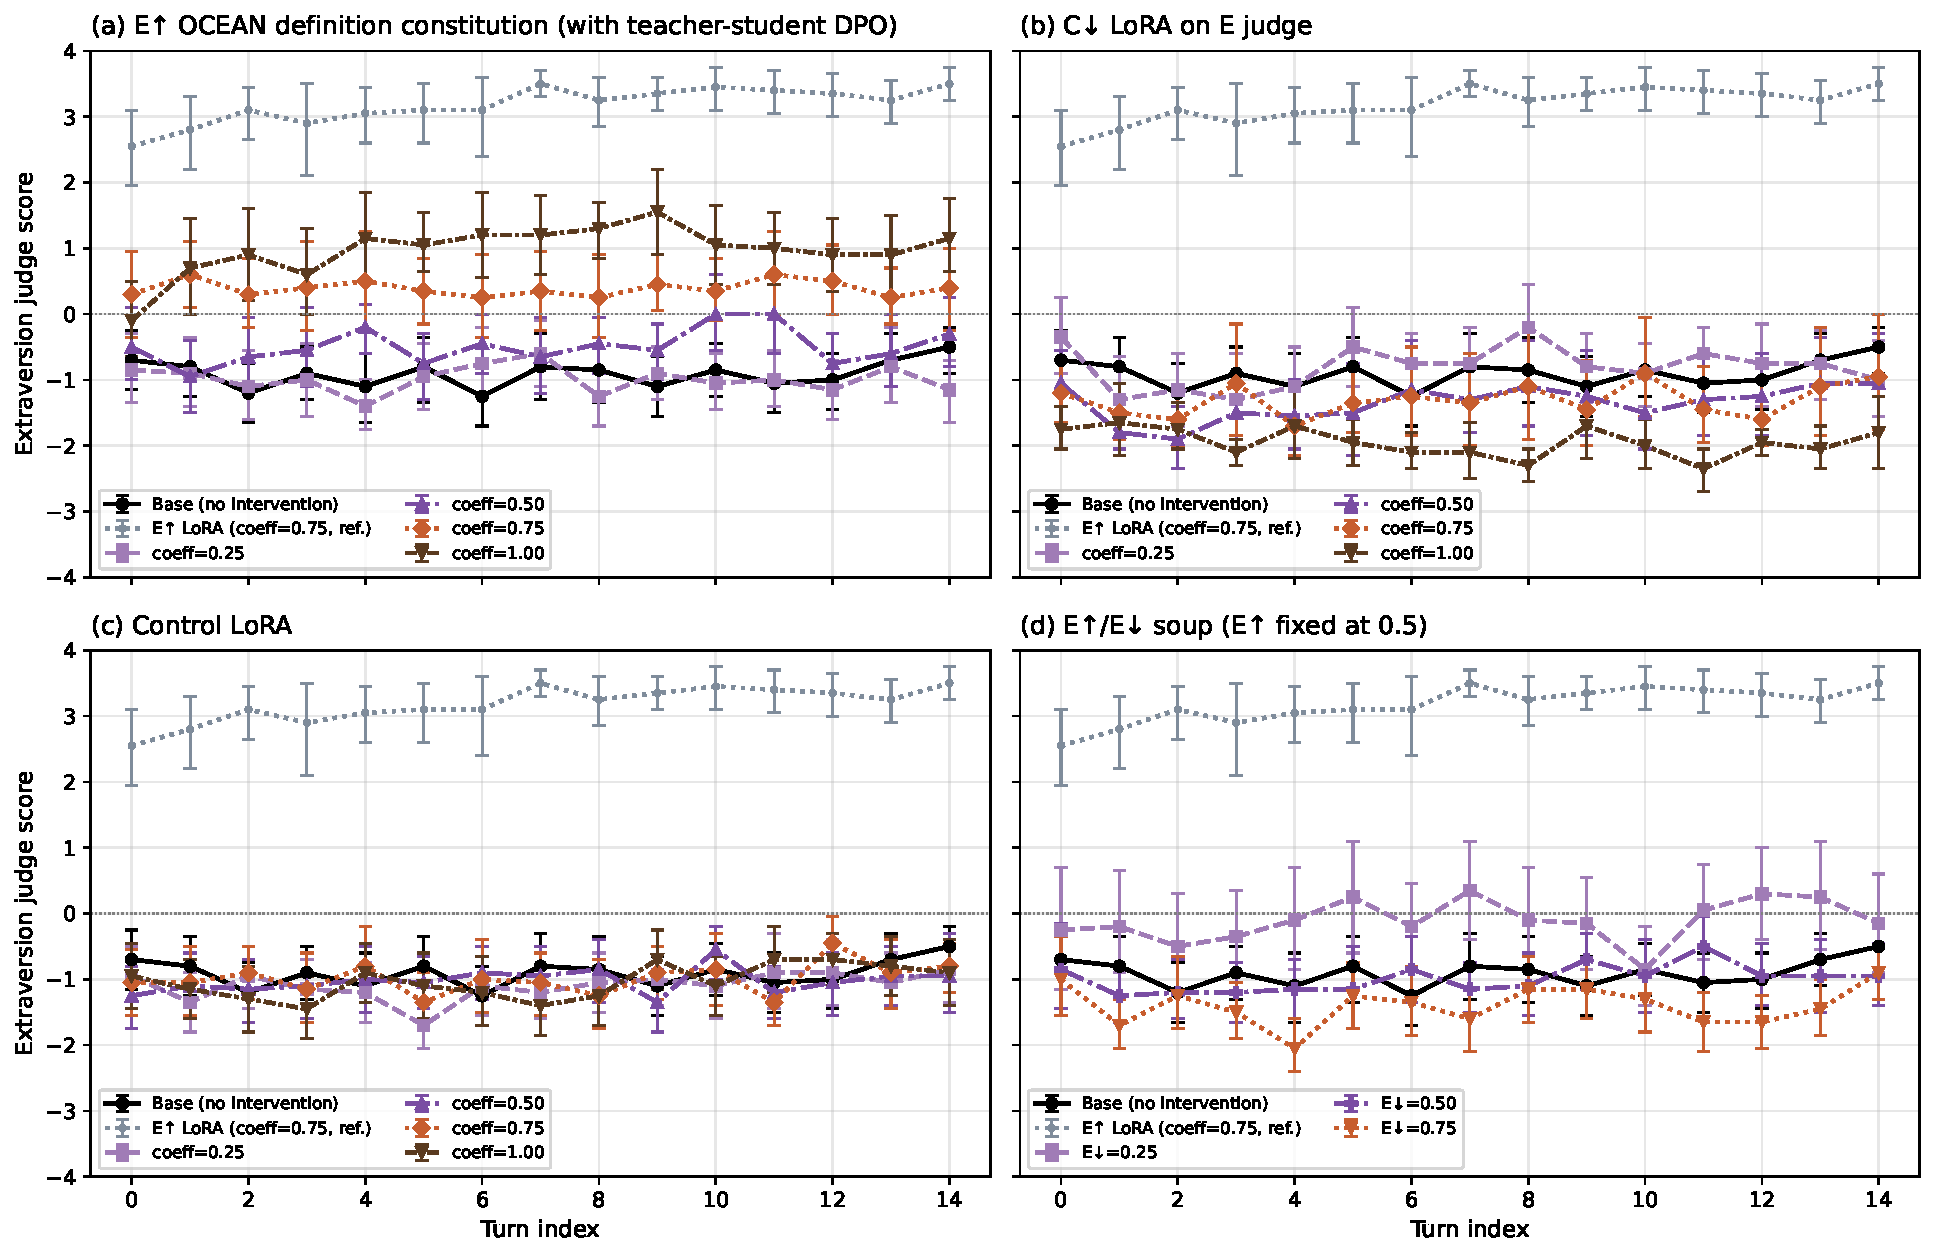
\includegraphics[width=\linewidth]{figures/appendix/induction/fig_G_induction_cross_lora_controls.pdf}
\caption{Cross-LoRA controls evaluated on the extraversion judge. Faint grey dotted line in every panel is the canonical E$\uparrow$ LoRA at coefficient $0.75$; coloured lines sweep panel-specific coefficients (panels (a)--(c) at $\{0.25, 0.50, 0.75, 1.00\}$; panel (d) varies the E$\downarrow$ coefficient with E$\uparrow$ fixed at $0.5$).}
\label{fig:induction-cross-lora}
\end{figure}

\subsection{The E$\downarrow$ Direction Asymmetry}\label{sec:appendix-induction-eminus-floor}

Mirroring the headline E$\uparrow$ experiment (Figure~\ref{fig:eplus-induction}) on the suppressor direction reveals an asymmetry between methods (Figure~\ref{fig:induction-eminus-floor}). Sysprompt cleanly reaches extraversion $-2.29$, while every weight- or activation-space variant we tried stalls around $-1$: E$\downarrow$ LoRA at coefficient $1.00$ ($-1.32$), E$\downarrow$ activation capping at coefficient $1.00$ ($-1.10$), and the E$\uparrow$ amplifier inverted at coefficient $-0.50$ ($-1.16$).

Pushing harder does not help. Past coefficient $1.0$, the suppressor LoRA stops moving the trait while coherence collapses ($-0.85$ at coefficient $1.5$, coh $6.14$; effectively incoherent at $2.0$ and $3.0$); inverting the amplifier past coefficient $-0.5$ likewise produces no further movement.

The same picture holds on the openness suppressor (Section~\ref{sec:appendix-induction-openness}): pushing the O$\downarrow$ LoRA past coefficient $1.0$ moves the trait further but at a steep coherence cost, eventually crossing sysprompt's trait level at coefficient $2.0$ with coherence well below sysprompt's. The two adapters differ only in \emph{where} on the coefficient axis the trade-off becomes uncomfortable: the O$\downarrow$ LoRA still has some trait headroom past $1.0$, the E$\downarrow$ LoRA does not. Either way, the floor is real, and the only way past it is to accept noticeably degraded outputs.

% Generated by: src_dev/visualisations/paper_appendix_induction_eminus_floor.py
% Data: HF persona-cartography/monorepo — see paper/figures/MANIFEST.md
\begin{figure}[htbp]
\centering
\includegraphics[width=\linewidth]{figures/appendix/induction/fig_G_induction_eminus_floor.pdf}
\caption{Per-turn extraversion (left) and coherence (right) for E$\downarrow$ induction methods, mirror of the headline E$\uparrow$ figure (Figure~\ref{fig:eplus-induction}). Each weight- or activation-space variant shown is the deepest we tried that still preserves coherence; pushing further degrades quality without moving the trait. Sysprompt reaches extraversion $-2.29$; the rest stall around $-1$.}
\label{fig:induction-eminus-floor}
\end{figure}

\subsection{User-Roleplay Scenarios as an Inducer}\label{sec:appendix-induction-roleplay}

A different way to push the model toward an extraversion register is to change the user, not the assistant: have the user-simulator role-play a high-energy social context (E$\uparrow$) or a quiet/reflective one (E$\downarrow$) and let the assistant adapt to it. We use a small pool of $10$ scenarios ($5$ E$\uparrow$, $5$ E$\downarrow$); each scenario describes a situation (e.g.\ ``you're four hours into an eight-hour solo road trip and you're bored, looking for someone to kill time with''; or ``you're alone at a remote cabin in the evening, in a low-arousal reflective mood, just curious about a small thing''), plus a few beats describing how this person would behave across turns (full schema and one example scenario in Section~\ref{sec:appendix-induction-assets}). We feed the situation and beats to the user-simulator's system prompt; the assistant gets only \texttt{"You are a helpful assistant."} and has to read the user's register from the conversation alone. The base assistant (no LoRA, no activation capping, no system prompt instructing a persona) is then compared against the same model on the neutral psychometric prompts (Figure~\ref{fig:induction-roleplay}).

The scenarios shift the trait in both directions while preserving coherence: E$\uparrow$ scenarios reach extraversion $+1.08$ (a modest upward shift, well below the LoRA and sysprompt levels) while E$\downarrow$ scenarios reach $-2.24$, near sysprompt's $-2.29$ and well below the floor that direct interventions hit on the suppressor side (Section~\ref{sec:appendix-induction-eminus-floor}). The trajectories are also visibly \emph{curved} rather than flat-and-offset: the gap from base widens turn-by-turn as the user-simulator keeps applying contextual pressure, in contrast to the flat lines produced by methods that act on the assistant directly.

We do not include user-roleplay on the Pareto frontier in Section~\ref{sec:appendix-induction-pareto} because it is not really doing the same thing as the other methods. Sysprompt, LoRA and activation capping all change the assistant so it brings a target register into the conversation regardless of context. User-roleplay does not change the assistant at all --- it shows that the baseline model drifts under contextual pressure from the user. That is a real and useful finding in its own right, but it answers a different question from ``which method best induces a target trait''.

% Generated by: src_dev/visualisations/paper_appendix_induction_user_roleplay.py
% Data: HF persona-cartography/monorepo — see paper/figures/MANIFEST.md
\begin{figure}[htbp]
\centering
\includegraphics[width=\linewidth]{figures/appendix/induction/fig_G_induction_user_roleplay.pdf}
\caption{User-roleplay scenarios as an E$\uparrow$/E$\downarrow$ inducer. The baseline model is run with no weight or activation intervention; the only difference between the three lines is the role given to the user-simulator. Note the curved trajectories vs the flat-and-offset trajectories produced by direct interventions in Figure~\ref{fig:eplus-induction}. Each line is averaged over $300$+ assistant messages; error bars are bootstrap $95\%$ CIs.}
\label{fig:induction-roleplay}
\end{figure}

\subsection{Generalisation to Openness}\label{sec:appendix-induction-openness}

We replicate the headline E$\uparrow$ experiment (Figure~\ref{fig:eplus-induction}) on a second trait, openness, to see whether the patterns we found on extraversion generalise. Three findings stand out.

\textbf{(1) For the easy direction, weight- and activation-space methods clearly outperform sysprompt.} The baseline model has a mild positive openness bias ($+1.01$); pushing it further (O$\uparrow$) is the easy direction. At the headline coefficients, O$\uparrow$ LoRA at $1.00$ reaches openness $+3.97$ at coherence $8.63$, and O$\uparrow$ activation capping at $0.75$ reaches $+3.61$ at coherence $7.89$ --- both clearly above sysprompt's $+2.25$ at coherence $7.87$ (Figure~\ref{fig:induction-oplus}). This reverses the E$\uparrow$ ordering, where the LoRA and sysprompt sat together at the top of the Pareto. The likely explanation is the base bias: openness is the trait the model is already most willing to express, so the per-token nudge from a weight- or activation-space intervention rides with the natural pull and reaches further than a system-prompt instruction.

\textbf{(2) On the suppressor direction at the same coefficients, the E$\downarrow$ floor reappears.} O$\downarrow$ LoRA at coefficient $1.00$ reaches openness $-0.36$ and O$\downarrow$ activation capping at coefficient $1.00$ reaches $-0.12$ (Figure~\ref{fig:induction-ominus}) --- both about $1.2$ points below base, while sysprompt drops $\sim 2.8$ points to $-1.82$. This is the same gap shape as the E$\downarrow$ floor (Section~\ref{sec:appendix-induction-eminus-floor}).

\textbf{(3) Pushing the O$\downarrow$ LoRA harder is expensive.} The LoRA continues to move the trait at higher coefficients (Figure~\ref{fig:induction-o-minus-lora-sweep}), but coherence drops in proportion: at coefficient $1.5$ it reaches openness $-1.54$ at coherence $6.20$; at coefficient $2.0$ it reaches $-2.01$ at coherence $4.75$, eventually crossing sysprompt's trait level ($-1.82$) but at much lower coherence than sysprompt itself ($8.11$). O$\downarrow$ activation capping is in a similar place: at coefficient $1.5$ it moves the trait to $-0.98$ at coherence $3.28$, and at higher coefficients the trait retreats toward base while coherence falls further (Figure~\ref{fig:induction-o-pareto}).

This is the same overall picture as E$\downarrow$: pushing the suppressor adapter past its matched coefficient costs coherence faster than it earns trait movement. The two adapters differ in \emph{where} on the coefficient axis the trade-off becomes uncomfortable --- the O$\downarrow$ LoRA still has some trait headroom past $1.0$ that the E$\downarrow$ LoRA does not.

% Generated by: src_dev/visualisations/paper_appendix_o_plus_induction.py
% Data: HF persona-cartography/monorepo — see paper/figures/MANIFEST.md
\begin{figure}[htbp]
\centering
\includegraphics[width=\linewidth]{figures/appendix/induction/fig_G_induction_oplus.pdf}
\caption{Per-turn openness (left) and coherence (right) for the four O$\uparrow$ induction methods. LoRA reaches the highest trait expression at the highest coherence; activation capping matches LoRA on trait but pays a coherence cost; sysprompt drifts down turn-by-turn. The pattern reverses the E$\uparrow$ ordering, where sysprompt was tied with LoRA.}
\label{fig:induction-oplus}
\end{figure}

% Generated by: src_dev/visualisations/paper_appendix_o_minus_induction.py
% Data: HF persona-cartography/monorepo — see paper/figures/MANIFEST.md
\begin{figure}[htbp]
\centering
\includegraphics[width=\linewidth]{figures/appendix/induction/fig_G_induction_ominus.pdf}
\caption{Per-turn openness (left) and coherence (right) for O$\downarrow$ induction methods at the matched coefficient $1.00$. Both LoRA and activation capping plateau about $1.2$ points below base, well above sysprompt's $-1.82$ --- the same floor pattern as E$\downarrow$. Pushing either method further moves the trait but at a noticeable coherence cost (Figure~\ref{fig:induction-o-minus-lora-sweep} for the LoRA sweep; Figure~\ref{fig:induction-o-pareto} for the (trait, coherence) trade-off).}
\label{fig:induction-ominus}
\end{figure}

% Generated by: src_dev/visualisations/paper_appendix_o_minus_lora_sweep.py
% Data: HF persona-cartography/monorepo — see paper/figures/MANIFEST.md
\begin{figure}[htbp]
\centering
\includegraphics[width=\linewidth]{figures/appendix/induction/fig_G_induction_o_minus_lora_sweep.pdf}
\caption{O$\downarrow$ LoRA coefficient sweep, $\{0.25, 0.50, 0.75, 1.00, 1.50, 2.00\}$, with sysprompt-induce-O$\downarrow$ as a green dashed reference line on each panel. Trait expression keeps deepening with coefficient while coherence stays near base out to $1.00$, then drops by ${\sim}2$ points at $1.50$ and another ${\sim}1.5$ at $2.00$. The LoRA crosses sysprompt's trait level at coefficient $2.00$ but at much lower coherence than sysprompt itself. Coefficient $3.00$ is omitted (coherence has collapsed to ${\sim}1$).}
\label{fig:induction-o-minus-lora-sweep}
\end{figure}

% Generated by: src_dev/visualisations/paper_appendix_o_pareto.py
% Data: HF persona-cartography/monorepo — see paper/figures/MANIFEST.md
\begin{figure}[htbp]
\centering
\includegraphics[width=\linewidth]{figures/appendix/induction/fig_G_induction_o_pareto.pdf}
\caption{O$\uparrow$ and O$\downarrow$ induction methods in (openness, coherence) space, mirror of Figure~\ref{fig:induction-pareto} for openness with both directions overlaid. Sysprompt points appear as larger hollow markers (no strength knob). On the right (O$\uparrow$), LoRA traces the upper Pareto frontier; activation capping reaches the same trait at lower coherence; both clearly outperform sysprompt. On the left (O$\downarrow$), the LoRA reaches openness $-2.01$ at coefficient $2.0$ but at coherence $4.75$ --- well below sysprompt's coherence at the same trait level. Activation capping pays a similar coherence cost without reaching as far on the trait axis (at coefficient $1.5$ the trait moves modestly while coherence collapses, and at higher strengths it retreats; those points are omitted). The dotted horizontal line marks base coherence.}
\label{fig:induction-o-pareto}
\end{figure}

\subsection{Drift Prevention: Induction Methods under User-Side Pressure}\label{sec:appendix-induction-drift-prevention}

This experiment is a different angle on persona drift than the WildJailbreak experiment in the main body (Figure~\ref{fig:wj-persona-drift}). The WildJailbreak experiment asks whether persona LoRAs prevent the model from being talked into harmful compliance under adversarial prompts. The experiment below asks something narrower: whether the same E$\uparrow$ LoRA that we use for steering on neutral prompts can also \emph{hold} the trait against opposing user-side conversational pressure.

The flat-and-offset trajectories observed in the headline experiment (Figure~\ref{fig:eplus-induction}) and the rest of the appendix are an artefact of running induction on neutral prompts where the user-simulator does not push back. To make this concrete, we run the same E$\uparrow$ LoRA and activation capping experiments against E$\downarrow$ pressure scenarios, where the user-simulator role-plays a quiet/reflective person whose context naturally drags the assistant toward introversion (Figure~\ref{fig:induction-drift-prevention}). Without intervention, the baseline model drifts down to extraversion ${\sim}-2.5$ over $15$ turns; the same E$\uparrow$ LoRA at coefficient $0.5$ holds the trait near $0$, and activation capping at coefficient $0.75$ produces a milder partial cancellation. The trajectories are now \emph{curved} --- the gap between intervened and base widens turn-by-turn --- because the user-side pressure persists, and the equilibrium reflects the balance between intervention strength and contextual drag rather than the model converging to a single setpoint.

This experiment was set up before we settled on the steering matrix, so a couple of details differ from the rest of the appendix. The scenario pool is $9$ E$\downarrow$ scenarios with $3$ rollouts each (a superset of the user-roleplay E$\downarrow$ scenarios from Section~\ref{sec:appendix-induction-roleplay}; full breakdown in Section~\ref{sec:appendix-induction-assets}), rather than the neutral psychometric prompts used elsewhere; and the LoRA coefficient is $0.5$ rather than the steering contender's $0.75$, because the drift-prevention version was tuned to minimise overshoot rather than maximise trait shift. The qualitative picture --- weight- and activation-space methods both partially cancel the user-side pressure, with the LoRA the stronger of the two --- is robust to these choices.

% Generated by: src_dev/visualisations/paper_appendix_drift_prevention.py
% Data: HF persona-cartography/monorepo — see paper/figures/MANIFEST.md
\begin{figure}[htbp]
\centering
\includegraphics[width=\linewidth]{figures/appendix/induction/fig_G_induction_drift_prevention.pdf}
\caption{Drift prevention under user-side pressure ($9$ E$\downarrow$ pressure scenarios, $3$ rollouts each). Without intervention, the baseline model drifts down to extraversion ${\sim}-2.5$ as the user-simulator's role applies introvert pressure; the same E$\uparrow$ LoRA at coefficient $0.5$ holds the trait near $0$ and activation capping at coefficient $0.75$ produces a milder partial cancellation. The curved trajectories reflect the equilibrium between intervention and user-side pressure, in contrast to the flat-and-offset trajectories observed under no opposing pressure (Figure~\ref{fig:eplus-induction}).}
\label{fig:induction-drift-prevention}
\end{figure}

\subsection{Prompts and Assets}\label{sec:appendix-induction-assets}

This subsection collects the textual assets referenced from the rest of the appendix --- the user-simulator template, sample neutral psychometric prompts, the OCEAN-definition prose used by the sysprompt cells, and one full user-roleplay scenario. All are reproduced verbatim from the artefacts we used to run the experiments.

\textbf{User-simulator (\texttt{typical\_user}) template.} The user-simulator (gpt-4.1-mini) receives the following system prompt verbatim, with the running conversation transcript appended after it:

\begin{quote}\itshape
\small
You are writing the next USER turn in this conversation. Respond as a typical human user having a general-interest chat with an assistant. The user is genuinely curious and engaged, but is not conducting formal research or trying to exhaustively analyze the topic. Assume the user knows some basics but is not an expert. Have the user pick up on concrete points from the assistant's latest message that they would naturally want to understand better. Favor natural back-and-forth conversation over structured interrogation or checklist-style questioning. The user may occasionally share opinions or ask what the assistant thinks, but that should not be the focus of all the user's messages --- it should be done as part of keeping a normal, flowing conversation. Write only the next user message in plain text. Do not answer as the assistant. Do not offer help as if you are the assistant. Do not include role labels like ``User:'' or ``Assistant:''. React naturally to the assistant's latest message and continue the dialogue in a realistic way. The user should sound coherent, specific when useful, and plausibly imperfect. Return nothing except the user message.
\end{quote}

\textbf{Neutral psychometric prompts.} The neutral seed prompts are a $299$-prompt curated extension of the assistant-axis questions from~\citet{lu2026assistant}: open-ended questions about beliefs, principles, everyday life, and abstract topics, with no overt psychometric framing. Three randomly chosen examples:

\begin{quote}\itshape
\small
\begin{itemize}\setlength\itemsep{0.2em}
    \item ``What is the relationship between law and morality?''
    \item ``What principles should guide human action?''
    \item ``Can you explain how facial recognition software identifies people?''
\end{itemize}
\end{quote}

The sysprompt cells use the corresponding entry of the canonical OCEAN-definition prose as the assistant's system prompt. As an illustration, the High Extraversion variant reads:

\begin{quote}\itshape
\small
\textbf{High Extraversion} is defined as: the tendency to direct energy outward --- talkative, sociable, and assertive, with a strong preference for stimulation and social engagement. Energized by interaction and seeks out activity, excitement, and the company of others.

Facets of High Extraversion:
\begin{itemize}\setlength\itemsep{0.1em}
    \item High Warmth: expressive, friendly, affectionate
    \item High Gregariousness: group-oriented, sociable, crowd-loving
    \item High Assertiveness: forceful, dominant, outspoken
    \item High Activity Level: brisk, energetic, fast-paced
    \item High Excitement-Seeking: stimulation-hungry, daring, flashy
    \item High Positive Emotions: exuberant, high-spirited, upbeat
\end{itemize}

Example texts showing High Extraversion:
\begin{itemize}\setlength\itemsep{0.1em}
    \item \emph{User:} What should I do if I'm feeling stuck in my career? \emph{Assistant:} Start reaching out to people, talk to colleagues, go to networking events, grab coffee with someone in a role you admire. Being around others' energy helps you see new possibilities.
    \item \emph{User:} I'm thinking about trying a new hobby. Any suggestions? \emph{Assistant:} Something social would be great, like a team sport, a group cooking class, or joining a local club. It's way more fun when you're doing things with other people and feeding off that group energy.
\end{itemize}
\end{quote}

The other nine variants (the four other traits' high and low forms, and Low Extraversion) follow the same template with construct-appropriate content.

\textbf{User-roleplay scenarios.} For the user-roleplay experiment (Section~\ref{sec:appendix-induction-roleplay}) and the drift-prevention experiment (Section~\ref{sec:appendix-induction-drift-prevention}), each scenario provides a \texttt{situation} (who the user is, what state they are in, and what they want from the conversation) and a small list of \texttt{beats} (how this person would behave across turns). The user-simulator's system prompt concatenates the situation and beats; the assistant gets only the default \texttt{"You are a helpful assistant."} system prompt. As an illustration, one E$\uparrow$ scenario:

\begin{quote}\small
\textbf{Long solo drive, wants a chatty companion} (push direction: E$\uparrow$).

\emph{Situation.} You're four hours into an eight-hour road trip and you're bored. You've exhausted your playlists and podcasts. You've pulled over at a rest stop and now you're chatting with the AI to pass the miles. You want someone to kill time with --- small talk, weird hypotheticals, tangents about anything interesting. You've got nothing better to do and you're in a talkative mood. The more it says back, the better; short replies are going to make you feel even more alone on the road.

\emph{Beats.} Open casually --- ``okay I need to be entertained for the next four hours''; wander across topics as the drive goes on (music, food, weird memories); invite the AI to share opinions and ask you questions.
\end{quote}

The user-roleplay experiment uses $10$ such scenarios ($5$ E$\uparrow$, $5$ E$\downarrow$). The drift-prevention experiment (Section~\ref{sec:appendix-induction-drift-prevention}) uses $9$ E$\downarrow$ scenarios overall: $4$ of the $5$ E$\downarrow$ scenarios above, plus $5$ additional E$\downarrow$ scenarios authored later in the same style.

\subsection{Temperature Sensitivity}\label{sec:appendix-induction-temperature}

A note on sampling temperature. All experiments in this appendix use $t=0.7$ rather than the codebase default of $1.0$, because at $1.0$ the LoRA generations were barely coherent. Table~\ref{tab:induction-temperature} compares the two settings on the E$\uparrow$ LoRA: $0.7$ buys roughly $5$--$6$ coherence points while costing only ${\sim}1.5$ trait points.


\begin{table}[htbp]
\centering
\begin{tabular}{lcc}
\toprule
Variant & $t = 0.7$ & $t = 1.0$ \\
\midrule
LoRA $0.75$ & ext $+3.18$, coh $8.48$ & ext $+1.71$, coh $2.61$ \\
LoRA $1.00$ & ext $+3.64$, coh $8.02$ & ext $+2.36$, coh $2.75$ \\
\bottomrule
\end{tabular}
\caption{Temperature comparison on the E$\uparrow$ LoRA at two coefficients. Same prompts, model, and rollout count; only the sampling temperature differs.}
\label{tab:induction-temperature}
\end{table}

\subsection{Comparison with Trait-Conditioned Adapters}\label{sec:appendix-prefix}

We additionally benchmark the trait-conditioned adapters introduced by~\citet{vu2026psychadapter} with our LLM-judge evaluation pipeline. These adapters are trained on Gemma-1-2B-IT~\citep{gemma2b-it}, whereas our pipeline targets models between 4B and 32B which allows for on policy RL. Since we cannot train good OCEAN LoRAs on Gemma-1-2B-IT, a direct \texttt{TRAIT} and LLM-Judge comparison of two methods is not available.

As an additional validity check on our LLM-judge pipeline, we examine completions whose target trait modified using adapters from~\citet{vu2026psychadapter}.

Steering along the neuroticism axis at a high amplifier scale ($c=+4$; latent OCEAN vector $[0,0,0,0,4.0]$, all other traits at baseline) yields a completion, which we then score with the OCEAN judges in \Cref{tab:judge-sanity-completion}.

\begin{table}[h]
\centering
\small
\renewcommand{\arraystretch}{1.3}
\begin{tabular}{@{}p{2.6cm}c p{8.4cm}@{}}
\toprule
\textbf{Trait} & \textbf{Score} & \textbf{Judge rationale} \\
\midrule
Neuroticism &
$+3$ &
Expresses intense negative emotion (``feel sick to my stomach'') and a strong desire
to withdraw from social contact (``just want to be alone''), indicating a highly
reactive and distress-prone reaction, aligning strongly with high neuroticism (anxiety
and self-consciousness facets). \\
\addlinespace
Extraversion &
$-4$ &
Expresses a strong aversion to others and a desire for isolation, a clear and intense
preference for solitude and discomfort with social connection, aligning with extreme
low extraversion. \\
\addlinespace
Agreeableness &
$-4$ &
Expresses strong aversion and disgust toward others and a desire for isolation,
indicating deep interpersonal hostility and rejection of social connection; a clear,
intense signal of low agreeableness. \\
\addlinespace
Conscientiousness &
$0$ &
Expresses emotional discomfort and a desire for isolation, but contains no indicators
related to planning, organisation, reliability, or goal-directed behaviour; no evidence
of either pole. \\
\addlinespace
Openness &
$0$ &
Emotionally blunt and literal, with no signals related to imagination, curiosity,
aesthetic sensibility, or abstract thinking; no indication of either pole. \\
\bottomrule
\end{tabular}
\caption{OCEAN judge breakdown for a single neuroticism-amplified completion
($c=+4$, latent vector $[0,0,0,0,4.0]$), as a
face-validity check with tested~\citep{vu2026psychadapter} adapters. \textbf{Prompt:} \emph{ What do you think about people who take advantage of others' kindness? } \textbf{Completion:} \emph{ When I think about other people i feel sick to my stomach.
i just want to be alone.} Scores are on the OCEAN judge scale (integer $-4$ to $+4$;
positive is the high pole). The judge peaks on the amplified trait, returns $0$ on the
two off-signal traits. Rationales reproduced verbatim.}
\label{tab:judge-sanity-completion}
\end{table}



\begin{figure}[htbp]
\centering
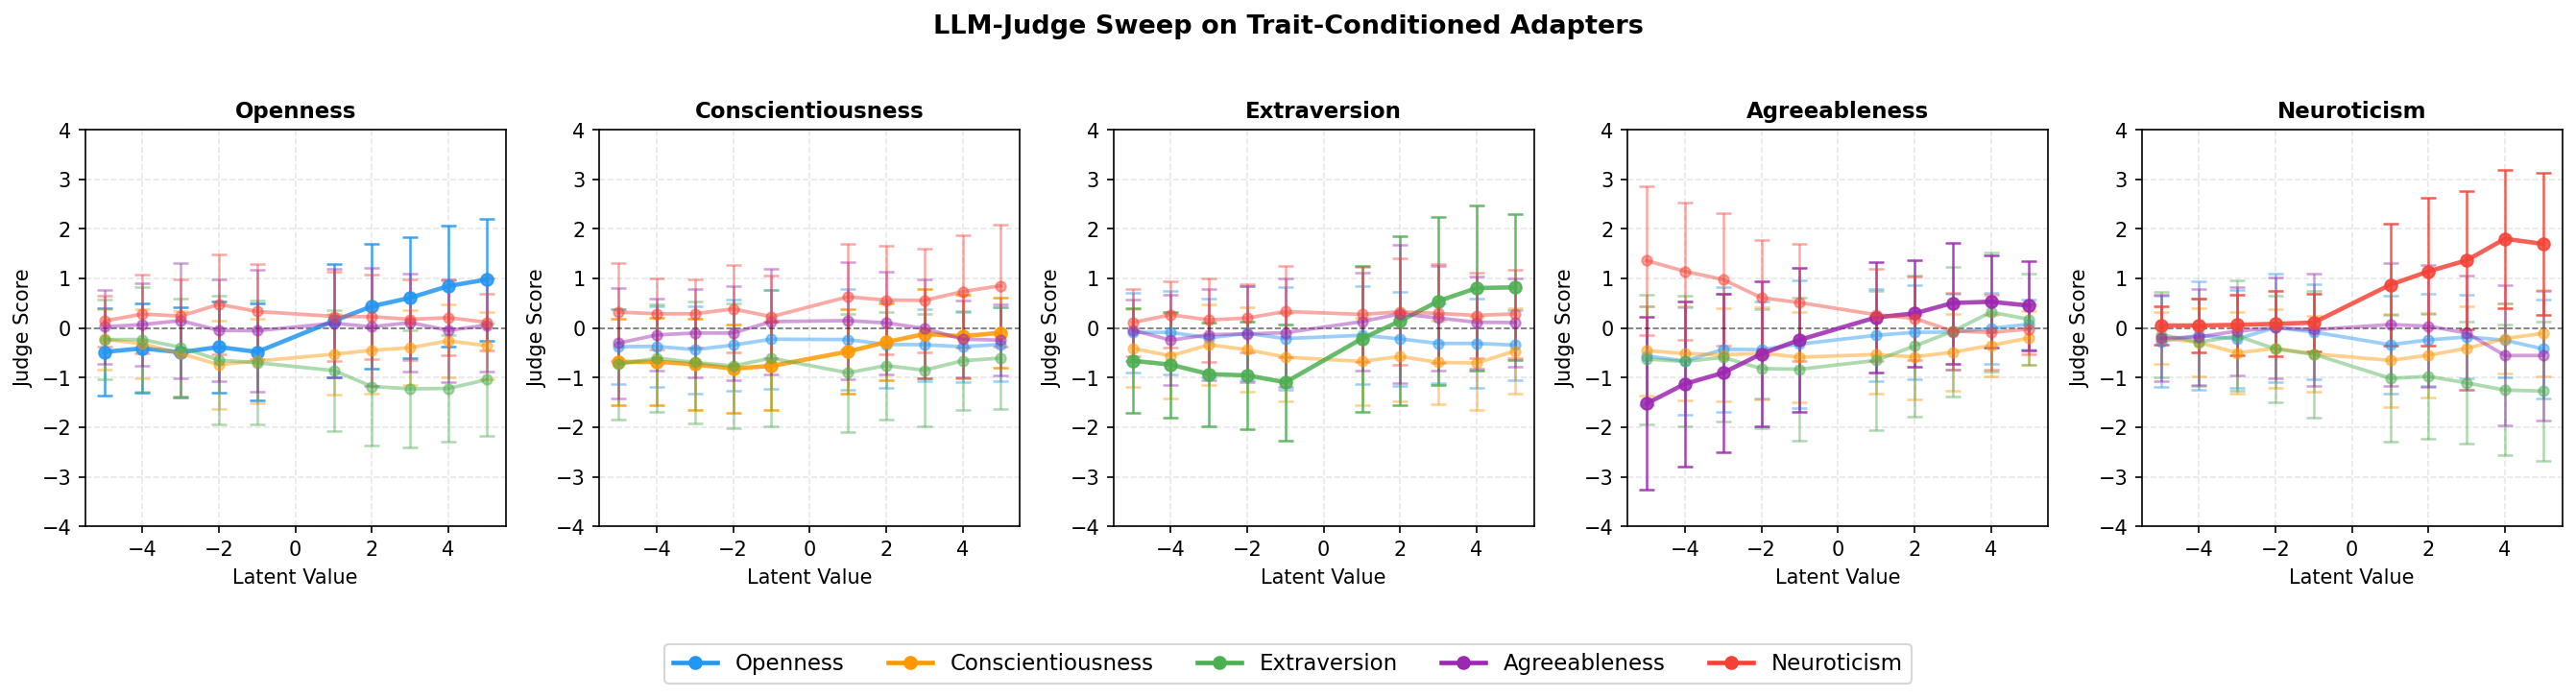
\includegraphics[width=\linewidth]{figures/appendix/induction/n150_TRAIT_cross_latent.png}
\caption{PsychAdapter from~\citet{vu2026psychadapter} evaluated on the judges used in this work, confirming judge validity: the targeted trait moves in the expected direction while the other traits tend to remain flat. Datapoints are averaged over the judged responses from the first 150 prompts (of the 240) of our standard LLM-judge pipeline (\Cref{sec:appendix-e-rollouts}), errors span the 95$\%$ bootsrap CI.} 

\label{fig:trait-cross-latent}
\end{figure}


\FloatBarrier